\documentclass[10pt,a4paper]{article}
\usepackage[margin=2.0cm]{geometry}
\usepackage[T1]{fontenc}
\usepackage{lmodern}
\usepackage{microtype}
\usepackage{booktabs}
\usepackage{longtable}
\usepackage{array}
\usepackage{amsmath,amssymb}
\usepackage{xcolor}
\usepackage{tikz}
\usetikzlibrary{arrows.meta,positioning}
\usepackage{pgfplots}
\usepgfplotslibrary{groupplots}
\pgfplotsset{compat=1.18}
\usepackage{float}
\usepackage[hidelinks]{hyperref}
\usepackage{enumitem}
\usepackage{fancyhdr}
\definecolor{accent}{HTML}{1D4ED8}
\definecolor{tomotopycolor}{HTML}{D97706}
\definecolor{softgray}{HTML}{F3F4F6}
\hypersetup{
  colorlinks=true,
  linkcolor=accent,
  urlcolor=accent,
  citecolor=accent,
  pdftitle={Neural MS2LDA: A One-Pass Deep Topic Model for Mass2Motif Discovery}
}
\newcommand{\StudySeed}{42}
\newcommand{\StudyTopics}{1000}
\newcommand{\StudyThreads}{6}
\newcommand{\FinalEpoch}{40}
\newcommand{\SourceSpectra}{41568}
\newcommand{\RetainedSpectra}{38888}
\newcommand{\TrainingSpectra}{27222}
\newcommand{\ValidationSpectra}{3889}
\newcommand{\TestSpectra}{7777}
\newcommand{\VocabularySize}{21233}
\newcommand{\TomotopyTrainingIterations}{750}
\newcommand{\NeuralValidationOptimized}{843}
\newcommand{\TomotopyValidationOptimized}{607}
\newcommand{\NeuralValidationEvaluable}{429}
\newcommand{\TomotopyValidationEvaluable}{206}
\newcommand{\NeuralValidationUseful}{268}
\newcommand{\TomotopyValidationUseful}{138}
\newcommand{\NeuralValidationSOS}{0.6507}
\newcommand{\TomotopyValidationSOS}{0.6761}
\newcommand{\NeuralValidationMedianSOS}{0.6441}
\newcommand{\TomotopyValidationMedianSOS}{0.6854}
\newcommand{\NeuralTestOptimized}{843}
\newcommand{\TomotopyTestOptimized}{607}
\newcommand{\NeuralTestEvaluable}{567}
\newcommand{\TomotopyTestEvaluable}{333}
\newcommand{\NeuralTestUseful}{347}
\newcommand{\TomotopyTestUseful}{186}
\newcommand{\NeuralTestSOS}{0.6369}
\newcommand{\TomotopyTestSOS}{0.6369}
\newcommand{\NeuralTestMedianSOS}{0.6333}
\newcommand{\TomotopyTestMedianSOS}{0.6145}
\newcommand{\NeuralCoverage}{84.3\%}
\newcommand{\TomotopyCoverage}{60.7\%}
\newcommand{\CoveragePointDelta}{23.6}
\newcommand{\ValidationOptimizedDelta}{236}
\newcommand{\ValidationEvaluableDelta}{223}
\newcommand{\ValidationUsefulDelta}{130}
\newcommand{\TestEvaluableDelta}{234}
\newcommand{\TestUsefulDelta}{161}
\newcommand{\NeuralValidationUsefulShare}{62.5\%}
\newcommand{\TomotopyValidationUsefulShare}{67.0\%}
\newcommand{\NeuralTestUsefulShare}{61.2\%}
\newcommand{\TomotopyTestUsefulShare}{55.9\%}
\newcommand{\NeuralFitMinutes}{35.8}
\newcommand{\TomotopyFitMinutes}{76.0}
\newcommand{\CoreFitRatio}{2.12}
\newcommand{\NeuralActiveTopics}{344}
\newcommand{\NeuralMedianEffectiveTopics}{6.43}
\newcommand{\NeuralValidationNLL}{8.8320}
\newcommand{\TomotopyValidationNLL}{9.6622}
\newcommand{\ValidationNLLDelta}{0.8302}
\newcommand{\NeuralTestNLL}{8.8412}
\newcommand{\TomotopyTestNLL}{9.7569}
\newcommand{\TestNLLDelta}{0.9158}
\newcommand{\WarmBatchSize}{128}
\newcommand{\NeuralWarmRate}{9093.9}
\newcommand{\TomotopyWarmRate}{30.0}
\newcommand{\WarmSpeedRatio}{302.6}

\pagestyle{fancy}
\fancyhf{}
\setlength{\headheight}{14pt}
\setlength{\headsep}{18pt}
\lhead{Neural MS2LDA}
\rhead{Seed \StudySeed, $K=\StudyTopics$, \StudyThreads{} CPU threads}
\cfoot{\thepage}
\setlist{nosep,leftmargin=*}
\newcommand{\softmax}{\operatorname{softmax}}
\newcommand{\normalize}{\operatorname{normalize}}
\newcommand{\stopgrad}{\operatorname{stopgrad}}
\tikzset{
  modelnode/.style={
    draw=black!55,
    rounded corners=2pt,
    align=center,
    minimum height=1.15cm,
    inner sep=3pt,
    font=\scriptsize
  },
  dataflow/.style={-{Latex[length=2.1mm]},line width=0.55pt,draw=black!70},
  trainflow/.style={
    -{Latex[length=2.1mm]},
    dashed,
    line width=0.55pt,
    draw=red!70!black
  },
  pipelinebox/.style={
    draw=black!55,
    fill=softgray,
    rounded corners=2pt,
    align=center,
    minimum height=1.35cm,
    text width=0.135\textwidth,
    inner sep=3pt,
    font=\scriptsize
  }
}

\title{Neural MS2LDA:\\
A One-Pass Deep Topic Model for Mass2Motif Discovery}
\author{}
\date{}

\begin{document}
\maketitle

\begin{abstract}
Mass2Motif discovery requires a model to explain held-out spectral evidence
while retaining a broad inventory of chemically interpretable fragment and
neutral-loss patterns. We present a neural probabilistic topic model in which
one sparse top-2 routing pass replaces iterative document-level inference.
Fixed, train-only token features and learned topic prototypes define both the
router and the topic--word decoder. Fragment and neutral-loss channels receive
equal probability mass, while balanced assignments, positive-NPMI structure,
and prototype separation address topic collapse. The architecture has 167,168
learned parameters and is optimized with alternating router and topic updates
over complete spectra. We compare Neural MS2LDA with Tomotopy LDA using the same
\StudyTopics{} topics, seed \StudySeed, \StudyThreads{} CPU threads, scaffold
split, and leakage-filtered MAG protocol. On validation, the neural model
produces \NeuralValidationOptimized{} optimized motifs and
\NeuralValidationUseful{} useful high-confidence motifs, versus
\TomotopyValidationOptimized{} and \TomotopyValidationUseful{} for Tomotopy.
On test, the corresponding useful-motif counts are \NeuralTestUseful{} and
\TomotopyTestUseful{}. Tomotopy has higher validation mean structure overlap
score (SOS), while test mean SOS is tied at four decimals. The result is
therefore a breadth--purity trade-off rather than uniform superiority. Recorded
core fitting time is lower for the neural model
(\NeuralFitMinutes{} versus \TomotopyFitMinutes{} minutes). This is a
single-dataset, single-seed research
comparison, not a claim that the neural model should replace the production
backend.
\end{abstract}

\section{Introduction}

MS2LDA represents tandem mass spectra as documents, fragment and neutral-loss
tokens as words, and recurrent co-occurrence patterns as Mass2Motifs
\cite{vanderhooft2016}. A useful large-scale model must do more than minimize a
predictive loss: it should retain many distinct motifs, assign spectra
confidently enough for motif-level analysis, and support chemical annotation
\cite{torresortega2026}.

Conventional latent Dirichlet allocation (LDA) estimates a new document's topic
mixture by iterative local inference \cite{blei2003}. Amortized neural inference
can replace that loop with a learned mapping, but a model with 1,000 topics can
collapse: a small subset of topics absorbs most probability mass, several
prototypes become near-duplicates, or learned topics ignore observed token
co-occurrence. Mass-spectrometry vocabularies introduce another bias. If
fragment and neutral-loss channel evidence is summed, the larger channel gains
mass simply because it contains more tokens, even when its mean logit is no
better.

We address these problems with one shared prototype geometry. It defines a
fragment/loss-balanced topic--word distribution and a contextual top-2 router
whose aggregated assignments form the document mixture in one pass. The
training objective combines full-spectrum likelihood with safeguards against
usage, geometric, and co-occurrence collapse. This report states the complete
model and evaluation protocol directly.

\section{Relation to neural topic models and contribution}

The broad ingredients of Neural MS2LDA have established precedents. Neural
Variational Document Models introduced an inference network that maps a bag of
words to a continuous stochastic document representation \cite{miao2016}. AVITM and
ProdLDA subsequently demonstrated one-pass amortized topic inference, discussed
component collapse explicitly, and replaced LDA's word-level mixture with a
product of experts \cite{srivastava2017}. The Embedded Topic Model (ETM)
parameterizes topic--word natural parameters with inner products between topic
and word embeddings \cite{dieng2020}. The Neural Sinkhorn Topic Model (NSTM)
also learns document-topic weights and cosine topic--word costs in an embedding
space, but trains them by minimizing an optimal-transport objective
\cite{zhao2021}. Contextualized topic models and FASTopic further show how
pretrained document representations can enter neural topic discovery
\cite{bianchi2021,wu2024}.

Neural MS2LDA is related to those models, but it is not a VAE, an ETM replica,
or an NSTM replica. It contains no sampled document latent variable, posterior
family, or KL term. Instead, a spectrum mixture is constructed directly by
aggregating sparse, contextual token routes. The same prototypes parameterize
those routes and the probabilistic decoder, while Sinkhorn supplies detached
balanced training targets rather than the main generative or transport
objective. Table~\ref{tab:lineage} makes the distinction explicit.

\begin{table}[ht]
  \centering
  \scriptsize
  \setlength{\tabcolsep}{5pt}
  \renewcommand{\arraystretch}{1.12}
  \begin{tabular}{@{}>{\raggedright\arraybackslash}p{0.15\textwidth}
    >{\raggedright\arraybackslash}p{0.21\textwidth}
    >{\raggedright\arraybackslash}p{0.25\textwidth}
    >{\raggedright\arraybackslash}p{0.30\textwidth}@{}}
    \toprule
    Model family & Document-topic inference & Topic--word construction &
    Principal distinction from Neural MS2LDA \\
    \midrule
    LDA / Tomotopy \cite{blei2003,tomotopy} &
    Iterative inference for each new document &
    Free categorical topic--word distributions &
    Neural MS2LDA amortizes inference into one neural pass and shares one
    geometry between routing and decoding. \\

    NVDM / AVITM / ProdLDA \cite{miao2016,srivastava2017} &
    Document-level neural variational posterior &
    Bag-of-words decoder; ProdLDA mixes in natural-parameter space &
    Neural MS2LDA deterministically aggregates token routes and has no sampled
    posterior, prior-matching KL, or reparameterization step. \\

    ETM \cite{dieng2020} &
    Amortized variational document encoder &
    Topic and word embedding inner products &
    Neural MS2LDA shares the geometric decoder idea, but its prototypes also
    drive sparse token routing with leave-one-out spectrum context. \\

    NSTM \cite{zhao2021} &
    Neural document-topic map &
    Cosine embedding cost trained through optimal transport &
    Neural MS2LDA retains mixture likelihood; Sinkhorn only creates detached,
    balanced router targets. \\

    Contextual / transport embedding models \cite{bianchi2021,wu2024} &
    Pretrained document embedding or direct semantic-relation reconstruction &
    Neural decoder or learned topic/word embedding transport &
    Neural MS2LDA uses train-only SGNS token features and a lightweight pooled
    spectrum context; a pretrained spectrum encoder is future work. \\

    \textbf{Neural MS2LDA (this work)} &
    Count-weighted aggregation of contextual top-2 token routes &
    Shared cosine prototypes with fixed 50/50 fragment/loss normalization &
    Mass-spectrometry-specific coupling of token routing, document gating,
    channel-balanced decoding, and complementary anti-collapse objectives. \\
    \bottomrule
  \end{tabular}
  \caption{Architectural lineage. The claimed contribution is Neural MS2LDA's
  combined formulation and mass-spectrometry adaptation, not first use of
  amortization, embedding decoders, sparse routing, or Sinkhorn individually.}
  \label{tab:lineage}
\end{table}

Within this comparison, no preceding model combines token-level leave-one-out
spectrum context, shared router/decoder prototypes, a directly aggregated
top-2 document mixture, and fixed fragment/loss channel mass. The methodological
contribution claimed here is therefore this mass-spectrometry-specific
formulation and its evaluation against Tomotopy. It is not a claim that each
building block is new, nor a first-ever priority claim over the entire neural
topic-model literature.

\section{Dataset and benchmark construction}

\subsection{MS\texorpdfstring{$^{n}$}{n}Lib source, acquisition, and loading}

MS$^{n}$Lib is an open reference-standard library created from seven compound
collections using automated multi-stage fragmentation acquisition and processing.
The complete resource contains more than 2.3 million MS$^{n}$ spectra, including
more than 357,000 MS$^{2}$ spectra for 30,008 unique structures across both
ionization modes \cite{brungs2025}. The MS2LDA 2.0 study filtered its positive-mode
MS$^{n}$Lib material to construct a diverse reference-standard benchmark for
unsupervised substructure discovery \cite{torresortega2026}. We use that published
benchmark input rather than resampling the full MS$^{n}$Lib resource.

The exact paper assets are distributed in Zenodo record 20179680
\cite{msnlibdata}. The acquisition script downloads only \texttt{Data.zip} and
\texttt{model\_positive\_mode.zip}. It verifies the Zenodo-declared byte size and
MD5 of each archive, checks ZIP integrity and paths, extracts through a staging
directory, verifies the required files and writes an acquisition manifest. The
topic-model input is
\path{Data/Benchmark_MSn_Lib/Corinna_Library_filtered_positive.mgf}; the
positive-mode Spec2Vec model, embedding matrix, and SQLite spectral library are
loaded only by the downstream MAG evaluation. Thus known molecular structures
are used for leakage-safe splitting and chemical scoring, not as labels for
fitting either topic model.

At run time, \texttt{protocol.json} supplies paths relative to a user-provided
data root; absolute-path escape is rejected. The streaming MGF reader treats each
\texttt{BEGIN IONS}/\texttt{END IONS} block as one spectrum, parses peaks rather
than trusting \texttt{NUM\_PEAKS}, and requires a Universal Spectrum Identifier
(USI), feature identifier, SMILES, InChIKey, and precursor $m/z$. RDKit reparses
the SMILES and checks that its derived connectivity InChIKey agrees with the
deposited identifier. Figure~\ref{fig:data-pipeline} summarizes the hand-off from
the public deposit to the sparse matrices consumed by the models.

\begin{figure}[t]
\centering
\begin{tikzpicture}[node distance=0.34cm]
  \node[pipelinebox] (zenodo) {Zenodo 20179680\\two frozen archives};
  \node[pipelinebox,right=of zenodo] (verify) {resume download\\size, MD5, ZIP checks};
  \node[pipelinebox,right=of verify] (extract) {staged extraction\\required-file checks};
  \node[pipelinebox,right=of extract] (parse) {stream MGF\\metadata and peak validation};
  \node[pipelinebox,right=of parse] (split) {seed-42 grouped split\\train-only vocabulary};
  \node[pipelinebox,right=of split] (matrix) {SciPy CSR matrices\\held-out JSONL records};
  \draw[dataflow] (zenodo) -- (verify);
  \draw[dataflow] (verify) -- (extract);
  \draw[dataflow] (extract) -- (parse);
  \draw[dataflow] (parse) -- (split);
  \draw[dataflow] (split) -- (matrix);
\end{tikzpicture}
\caption{Reproducible MS$^{n}$Lib ingestion. The MGF supplies spectral documents;
the positive-mode Spec2Vec assets branch from the verified extraction only for
leakage-filtered MAG annotation.}
\label{fig:data-pipeline}
\end{figure}

\subsection{Spectrum processing, representation, and split}

The source MGF contains \SourceSpectra{} positive-mode spectra. Within each
spectrum, intensities are divided by the largest finite peak intensity. Peaks
outside $m/z\in(0,2000]$ or normalized intensity $[0.01,1]$ are discarded; if
more than 1,000 remain, the most intense peaks are kept, and spectra with fewer
than five retained peaks are dropped. This deterministic cleaning retains
\RetainedSpectra{} spectra.

Each physical peak generates a fragment word and, when the precursor-minus-peak
mass exceeds 0.01 Da, a neutral-loss word. Both masses are rounded to two decimal
places, producing tokens such as \texttt{frag@70.04} and \texttt{loss@162.05}, as
in MS2LDA 2.0 \cite{torresortega2026}. A peak with normalized intensity $I$ is
represented by $\operatorname{round}(100I)$ copies of each applicable word. The
result is a count-valued bag of spectral words, not a sequence and not a list of
structure labels.

Molecules are keyed by the connectivity block of the InChIKey. Cyclic molecules
are grouped by non-chiral Bemis--Murcko scaffold \cite{bemismurcko1996}; each
acyclic connectivity group remains intact. Groups are sorted by descending size
and assigned deterministically toward 70/10/20 train, validation, and test
targets using seed \StudySeed. The resulting matrices contain
\TrainingSpectra{} training, \ValidationSpectra{} validation, and \TestSpectra{}
test spectra, with zero compound or scaffold overlap. The vocabulary is then
constructed from training spectra only, requires document frequency at least
three, preserves first-seen training order, and contains \VocabularySize{}
fragment/loss tokens. Every split is written in that fixed column order as a
SciPy CSR count matrix.

For document-completion evaluation, the loader deterministically divides whole
physical peak groups 50/50. A fragment and the neutral loss derived from the same
peak therefore cannot fall on opposite sides. The observed half is renormalized
without consulting the withheld maximum; out-of-vocabulary held-out words are
recorded and excluded from the likelihood denominator. All learned parameters,
token features, vocabulary entries, and co-occurrence statistics use the
training partition only. Validation and test spectra use that fixed training
vocabulary and are evaluated as separate held-out splits.

\section{Neural MS2LDA architecture}

Neural MS2LDA must connect two directions of reasoning. Given a spectrum, it
must infer a small set of topics that explain the observed peaks; given a topic,
it must produce an explicit fragment/loss distribution that can be inspected as
a Mass2Motif. The subsections follow that forward path. They first define the
probabilistic contract, then construct token representations, place tokens and
topics in one shared geometry, and finally aggregate context-dependent token
routes into a document mixture.

Each piece addresses a separate requirement. Fixed train-only features give the
model co-occurrence information without using molecular labels. Shared
prototypes keep routing and decoding semantically aligned, while channel
balancing prevents the larger fragment or neutral-loss vocabulary from winning
by size alone. The contextual sparse router resolves tokens that have different
meanings in different spectra and replaces iterative document inference with one
neural pass. Together these pieces retain a conventional probabilistic
topic--word output while providing a differentiable spectrum--topic map.

\subsection{Model notation and overview}

Let $d\in\{1,\ldots,D\}$ index spectra, $w\in\{1,\ldots,V\}$ index the shared
fragment/loss vocabulary, and $k\in\{1,\ldots,K\}$ index topics. The count
$c_{dw}\geq0$ is the spectral-word multiplicity. The model returns a
document--topic distribution $\theta_d\in\Delta^{K-1}$ and a topic--word
distribution $\beta_k\in\Delta^{V-1}$, with
\begin{equation}
  p(w\mid d)=\sum_{k=1}^{K}\theta_{dk}\beta_{kw}.
  \label{eq:mixture}
\end{equation}

\subsection{Fixed token features}

Each token has a fixed feature vector $x_w\in\mathbb{R}^{50}$. Its first 48
coordinates are skip-gram negative-sampling (SGNS) embeddings trained only on
training documents \cite{mikolov2013}. For five epochs, eight count-weighted
positive pairs are sampled per document; each positive pair uses five negatives
drawn with probability proportional to corpus frequency raised to $0.75$.
Source embeddings are initialized uniformly on $[-0.5/48,0.5/48]$ and context
embeddings at zero. SparseAdam uses learning rate 0.01 and batches of 8,192
pairs. Source and context embeddings are averaged and normalized after the
fifth epoch. Two final one-hot coordinates mark fragment versus neutral loss.
The normalized SGNS vector and type indicators are concatenated and normalized
again. These are the complete token features used by the model; molecular
labels do not enter fitting.

\subsection{Shared topic geometry and balanced decoder}

This stage gives every spectral word and every topic a position in one learned
space. Sharing the space is important because the two directions of the topic
model must agree: the router assigns observed evidence to a topic, while the
decoder states which evidence that topic is expected to emit. If those two
parts used unrelated representations, a spectrum could be routed to a topic
whose word distribution described something else. The shared prototypes are
therefore the semantic bridge between one-pass inference and interpretable
Mass2Motifs.

A learned bias-free matrix $W\in\mathbb{R}^{128\times50}$ projects the fixed
features, and every topic has a learned prototype $q_k\in\mathbb{R}^{128}$:
\begin{equation}
  z_w=\normalize(Wx_w),\qquad \widehat q_k=\normalize(q_k).
\end{equation}
The matrix $W$ is initialized orthogonally. The same $z_w$ and $\widehat q_k$
are used by both decoder and router. Decoder
logits are temperature-scaled cosine similarities,
\begin{equation}
  \ell_{kw}=\frac{2\widehat q_k^\top z_w}{\tau_\beta},
  \qquad \tau_\beta=0.18.
  \label{eq:decoder-logits}
\end{equation}

Let $V_F$ and $V_L$ denote the fragment and neutral-loss vocabularies. Each
channel receives exactly one half of the topic probability mass, and a softmax
within that channel determines token rankings:
\begin{equation}
  \beta_{kw}=\frac{1}{2}
  \frac{\exp(\ell_{kw})}
       {\sum_{v\in V_{t(w)}}\exp(\ell_{kv})}.
  \label{eq:beta}
\end{equation}
Thus $\sum_w\beta_{kw}=1$, vocabulary size cannot change channel mass, rankings
within each channel are unchanged, and the channel correction adds no learned
parameter. The fixed split is needed because fragments and neutral losses are
two chemically useful views of the same peaks but can have very different
vocabulary sizes. A single global softmax could reward the larger channel merely
for having more candidate words. Giving each channel half of the mass removes
that size effect while leaving the model free to learn rankings within each
channel. The resulting $\beta_k$ is both the probabilistic decoder used in the
likelihood and the Mass2Motif spectrum supplied to MAG.

\subsection{Contextual top-2 router and document mixture}

The decoder answers ``what does topic $k$ contain?''; the router answers the
reverse question, ``which topics explain this spectrum?'' A fragment or loss can
occur in several chemical contexts, so its identity alone is insufficient. The
router combines three levels of evidence: the token embedding, the other words
in the same spectrum, and a pooled whole-spectrum summary. This lets the same
token support different topics in different spectra without running an
iterative inference procedure for each new document.

For spectrum $d$, define the count-weighted embedding sum
$s_d=\sum_w c_{dw}z_w$. For each non-zero token entry, the leave-one-out context
is
\begin{equation}
  \bar z_{d\setminus w}=
  \frac{s_d-c_{dw}z_w}{\max(\sum_v c_{dv}-c_{dw},1)}.
  \label{eq:context}
\end{equation}
A nonlinear context router transforms the concatenated token and context. Let
$W_c\in\mathbb{R}^{128\times256}$ denote its single learned bias-free matrix.
Then
\begin{align}
  e_{dw} &= \operatorname{GELU}
  \!\left(W_c[z_w;\bar z_{d\setminus w}]\right),\\
  h_{dw} &= \normalize\!\left(z_w+e_{dw}\right),
  \qquad u_d=\normalize(s_d).
  \label{eq:context-router}
\end{align}
The router matrix is initialized from $\mathcal N(0,0.01^2)$, so training begins
near the token geometry while retaining a nonlinear learned correction. The
model has 167,168 learned parameters: 6,400 in the token projection, 32,768 in
the context router, and 128,000 in the topic prototypes.
Local and document evidence are added before routing:
\begin{equation}
  a_{dwk}=h_{dw}^{\top}\widehat q_k+u_d^{\top}\widehat q_k,
  \qquad r^{\mathrm{soft}}_{dw}=\softmax_k(a_{dwk}/T).
  \label{eq:routing-logits}
\end{equation}
Only the two largest entries of $r^{\mathrm{soft}}_{dw}$ are retained and
renormalized to form $r^{\mathrm{hard}}_{dw}$. Training uses the straight-through
quantity
$r^{\mathrm{hard}}+r^{\mathrm{soft}}-\stopgrad(r^{\mathrm{soft}})$; inference
uses $r^{\mathrm{hard}}$ directly.

Count-weighted routed mass is $M_{dk}=\sum_w c_{dw}r_{dwk}$. The same
whole-spectrum score supplies a multiplicative document gate,
\begin{equation}
  g_{dk}=\softmax_k(u_d^\top\widehat q_k/T),\qquad
  \theta_{dk}=\frac{M_{dk}g_{dk}^{\gamma}}
  {\sum_jM_{dj}g_{dj}^{\gamma}},\qquad \gamma=0.75.
  \label{eq:theta}
\end{equation}
The gate is detached in Equation~\ref{eq:theta} during training, so it cannot
reduce the loss by sharpening itself; its document score still learns through
Equation~\ref{eq:routing-logits}. Multiplication preserves exact zero support
from token routing. If a spectrum has no routed mass, $\theta_d$ is explicitly
uniform. Equations~\ref{eq:routing-logits}--\ref{eq:theta} require one forward
pass and no per-spectrum optimization loop. Conceptually, contextual tokens cast
sparse topic votes, count aggregation combines those votes, and the document
gate checks whether the voted topics also fit the spectrum as a whole. Because
the gate only reweights routed mass, it cannot introduce a topic unsupported by
the token-level assignments.

The count-weighted completion loss implements Equation~\ref{eq:mixture}
exactly at non-zero target entries:
\begin{equation}
  \mathcal L_{\mathrm{comp}}(\theta,X)=
  -\frac{1}{\sum_{dw}c_{dw}}
  \sum_{dw}c_{dw}\log\!\left(\sum_k\theta_{dk}\beta_{kw}\right).
  \label{eq:completion}
\end{equation}
Sparse indexing avoids materializing the dense matrix $\theta\beta$ but does
not change its probabilities. Read from left to right, the complete forward path
is: fixed token features $\rightarrow$ learned token positions $\rightarrow$
context-dependent top-2 routes $\rightarrow$ one document mixture
$\rightarrow$ a mixture of topic-word distributions. The prototype bank is the
shared junction: it receives routing evidence from the left and defines the
decoder on the right. Figure~\ref{fig:model} shows this flow and separates it
from the training-only safeguards.

\begin{figure}[ht]
  \centering
  \begin{tikzpicture}[x=1cm,y=1cm]
    \node[modelnode,fill=blue!7,text width=2.05cm] (features) at (0,0) {
      Fixed token features\\
      $x_w\in\mathbb R^{50}$\\
      48 SGNS + 2 type};
    \node[modelnode,fill=blue!12,text width=2.05cm] (projection) at (2.55,0) {
      Learned projection\\
      $z_w=\normalize(Wx_w)$\\
      $\mathbb R^{50}\!\to\!\mathbb R^{128}$};
    \node[modelnode,fill=blue!12,text width=2.15cm] (context) at (5.35,0) {
      Leave-one-out context\\
      $\bar z_{d\setminus w}\in\mathbb R^{128}$\\
      Linear $256\!\to\!128$ + GELU};
    \node[modelnode,fill=blue!12,text width=2.15cm] (router) at (8.25,0) {
      Local + document scores\\
      soft route $\to$ top-2\\
      $r_{dw}\in\Delta^{999}$};
    \node[modelnode,fill=yellow!18,text width=2.2cm] (aggregate) at (11.25,0) {
      Count aggregation + gate\\
      $M_d\odot\stopgrad(g_d)^{0.75}$\\
      $\theta_d\in\Delta^{999}$};
    \node[modelnode,fill=green!12,text width=1.95cm] (mixture) at (14.15,0) {
      Completion model\\
      $p(w\mid d)$\\
      $=\sum_k\theta_{dk}\beta_{kw}$};

    \draw[dataflow] (features) -- (projection);
    \draw[dataflow] (projection) -- (context);
    \draw[dataflow] (context) -- (router);
    \draw[dataflow] (router) -- (aggregate);
    \draw[dataflow] (aggregate) -- (mixture);

    \node[modelnode,fill=violet!10,text width=2.8cm] (prototypes) at (8.25,-1.85) {
      One shared prototype bank\\
      $\widehat Q\in\mathbb R^{1000\times128}$\\
      initialized from distinct tokens};
    \node[modelnode,fill=violet!7,text width=2.65cm] (decoder) at (11.65,-1.85) {
      Channel-balanced decoder $\beta$\\
      inputs $z_w,\widehat q_k$; cosine logits\\
      $\tfrac12$ fragments + $\tfrac12$ losses};

    \draw[dataflow] (prototypes) -- node[right,font=\scriptsize] {router geometry} (router);
    \draw[dataflow] (prototypes) -- (decoder);
    \draw[dataflow] (decoder) -- (mixture);

    \node[font=\scriptsize\bfseries,text=red!70!black,anchor=west]
      at (-1.05,-3.75) {Training only};
    \node[modelnode,fill=red!4,text width=1.95cm] (sinkhorn) at (5.25,-3.75) {
      Temperature annealing\\and Sinkhorn usage targets};
    \node[modelnode,fill=red!4,text width=1.95cm] (separation) at (8.25,-3.75) {
      Eight-neighbour\\prototype separation};
    \node[modelnode,fill=red!4,text width=1.95cm] (npmi) at (11.65,-3.75) {
      Positive-NPMI\\co-occurrence graph};

    \draw[trainflow] (sinkhorn.north) to[out=90,in=180] (router.west);
    \draw[trainflow] (separation.north) -- (prototypes.south);
    \draw[trainflow] (npmi.north) -- (decoder.south);

    \node[font=\scriptsize,text=red!70!black,anchor=west,align=left,
      text width=1.9cm] at (13.05,-3.75) {
      Dashed paths are absent from held-out inference.};
  \end{tikzpicture}
  \caption{Complete Neural MS2LDA computation graph. Solid arrows form the one-pass
  forward model used at training and inference. The prototype bank branches to
  both the contextual router and the probabilistic decoder. Dashed red arrows
  show training-only collapse safeguards. Dimensions and channel normalization
  are part of the implemented architecture, not illustrative placeholders.}
  \label{fig:model}
\end{figure}

\section{Training objective and anti-collapse design}

Defining the forward model is not sufficient when \StudyTopics{} topics share
one learned space. Without coordinated learning, a few topics can absorb most
routes, several prototypes can become duplicates, or a decoder can assign high
probability to words that rarely co-occur. This section therefore separates two
training questions: how the router and decoder take turns learning from the same
completion objective, and how the model preserves a broad, coherent topic
inventory while they do so.

The first subsection describes the alternating router and topic blocks. This
schedule is needed because the projection and prototypes define both sides of
the model: changing the routes changes the evidence used to learn topics, while
changing the decoder changes what counts as a good route. The second subsection
collects safeguards with distinct jobs---initialization anchors topics,
temperature annealing moves from exploration to specialization, Sinkhorn resists
topic starvation, positive NPMI rewards observed co-occurrence, and prototype
separation resists duplication. Completion likelihood remains the predictive
anchor throughout. These mechanisms affect fitting only; the trained model still
uses the single forward path in Figure~\ref{fig:model}.

\subsection{Alternating full-spectrum optimization}

The projection and prototypes serve both routing and decoding, so learning one
side changes the target seen by the other. Alternating the updates makes that
coordination explicit: the router first learns where spectral evidence should
go while the current decoder is fixed, then the topic block learns what each
topic should emit while the current routes are fixed. The completion likelihood
is the common contract between the blocks. Alternation is a training schedule,
not an additional inference stage; a fitted model still uses the single forward
path in Figure~\ref{fig:model}.

Optimization alternates two gradient blocks using one AdamW optimizer. In the
\emph{router block}, $\beta$ is cached and detached. One full-spectrum route is
optimized with likelihood, Sinkhorn targets, and prototype separation:
\begin{equation}
  \mathcal L_{\mathrm{router}}=
  \mathcal L_{\mathrm{comp}}+\omega_S\mathcal L_{\mathrm{Sinkhorn}}
  +5\mathcal L_{\mathrm{sep}}.
  \label{eq:router-loss}
\end{equation}
For a mini-batch with $N$ routed entries, log-space Sinkhorn iteration projects
$\exp(a/\varepsilon)$, with $\varepsilon=0.05$, to detached targets $Q$ whose
rows sum to one and whose columns sum to $N/K$ \cite{cuturi2013,caron2020}.
$\mathcal L_{\mathrm{Sinkhorn}}$ is cross-entropy from $Q$ to
$\softmax(a/T)$. Sinkhorn is a training target only; it is not part of held-out
inference.

In the \emph{topic block}, routes are recomputed without gradients and held
fixed. Decoder geometry is then optimized with
\begin{equation}
  \mathcal L_{\mathrm{topic}}=
  \mathcal L_{\mathrm{comp}}+\mathcal L_{\mathrm{NPMI}}
  +5\mathcal L_{\mathrm{sep}},
  \label{eq:topic-loss}
\end{equation}
using the same full training spectra. A full router pass with batch size 128 is
followed by four topic-block updates with batch size 512 per epoch. Each
auxiliary loss is attached to the part whose failure it addresses: Sinkhorn
encourages the router to use the available topic capacity, positive NPMI makes
decoder words cohere according to observed co-occurrence, and prototype
separation discourages topics from becoming geometric duplicates. Completion
likelihood and separation appear in both blocks, keeping prediction and topic
identity coupled throughout training.

\subsection{Complementary anti-collapse terms}

The safeguards target complementary collapse modes: topic starvation,
incoherent word groups, and duplicate prototypes.
\begin{enumerate}
  \item \textbf{Deterministic initialization.} Seed \StudySeed{} selects
  \StudyTopics{} distinct projected training tokens uniformly without
  replacement, giving every initial prototype a concrete spectral-word anchor.

  \item \textbf{Annealed sparse routing.} Routing temperature falls linearly
  from 0.5 to 0.1 over 30 epochs. Early soft assignments permit exploration;
  later top-2 assignments specialize.

  \item \textbf{Balanced usage.} The Sinkhorn coefficient is 0.25 for the first
  ten epochs and then decreases linearly to 0.05 at epoch \FinalEpoch. It
  resists early winner-take-all collapse without forcing uniform usage at the
  end of training.

  \item \textbf{Train-only co-occurrence structure.} Binary training documents
  define a positive-NPMI graph. Tokens require document frequency at least ten,
  pair frequency at least three, and mutual membership among at most 16
  strongest neighbours. If $A$ is the resulting weighted sparse adjacency,
  the retained edge weight is
  \begin{equation}
    A_{wv}=\frac{\log[p(w,v)/(p(w)p(v))]}{-\log p(w,v)},
    \qquad A_{wv}>0,
  \end{equation}
  where probabilities are empirical document frequencies. Only mutual
  top-neighbour edges remain. The training loss is
  \begin{equation}
    \mathcal L_{\mathrm{NPMI}}=-\frac1K\sum_k
    \log\!\left(\sum_{wv}\beta_{kw}A_{wv}\beta_{kv}\right).
  \end{equation}
  This favours probability mass on training-supported token pairs.

  \item \textbf{Prototype separation.} For every prototype, the eight nearest
  other prototypes are penalized above cosine margin 0.3:
  \begin{equation}
    \mathcal L_{\mathrm{sep}}=\operatorname{mean}_{k,j}
    \left[\max(0,\widehat q_k^\top\widehat q_j-0.3)\right]^2.
  \end{equation}
  This detects geometric duplication that usage balance cannot detect.

  \item \textbf{Numerical controls.} PyTorch deterministic algorithms are
  required under the six-thread allowance. Non-finite losses or gradients stop
  training immediately, and gradient norm is clipped to 5.0. Training always
  runs to the predeclared epoch \FinalEpoch.
\end{enumerate}

AdamW uses learning rate $10^{-3}$, weight decay $10^{-4}$, and seed
\StudySeed. Table~\ref{tab:hyperparameters} lists the complete settings.

\section{Evaluation protocol}

\subsection{Comparator and timing boundary}

Tomotopy 0.13.0 \cite{tomotopy} is trained independently on the same training
matrix and never acts as a teacher. It uses $K=\StudyTopics$, scalar initial
$\alpha=0.6$ with optimization interval 10, $\eta=0.1$, seed \StudySeed,
\StudyThreads{} workers, and parallel scheme 3. Training advances in blocks of
50 to at most 5,000 iterations and stops when all of the last ten relative
perplexity changes are below 0.005. The recorded fit stops at
\TomotopyTrainingIterations{} iterations. Held-out Tomotopy mixtures use 100
iterations, \StudyThreads{} workers, parallel scheme 1, and independent-document
inference. The neural model has no corresponding iteration count because its
document mapping is amortized into one routing pass.

Reported fitting time is optimization-loop wall time. For the neural model it
excludes MGF processing, SGNS feature construction, co-occurrence graph
construction, initialization, and evaluation; for Tomotopy it excludes sparse
matrix expansion, model construction, and evaluation. This gives like-for-like
core fitting time but is not total workflow time.

Runtime is reported descriptively and is not a motif-quality metric. Warm
inference is reported separately because it measures resident models and already
prepared sparse batches; it is not end-to-end latency.

\subsection{Predictive, inventory, and chemical metrics}

No single number answers whether an unsupervised topic model is useful. The
benchmark therefore separates predictive fit, the size of the annotatable motif
inventory, and the chemical consistency of that inventory. Table~\ref{tab:metrics}
gives the reading rule for every headline metric.

\begin{table}[H]
\centering
\small
\begin{tabular}{@{}>{\raggedright\arraybackslash}p{0.21\textwidth}
                >{\raggedright\arraybackslash}p{0.47\textwidth}
                >{\raggedright\arraybackslash}p{0.22\textwidth}@{}}
\toprule
Metric & Calculation & Interpretation \\
\midrule
Completion NLL & Log loss on withheld in-vocabulary token counts after routing
the observed half-spectrum. & Lower is better predictive fit. \\
Optimized motifs & Topics for which MAG optimization retains at least one
fragment or loss. & Larger means a broader annotatable inventory. \\
MAG coverage & Optimized motifs divided by all $K=\StudyTopics$ topics. & A
percentage form of the optimized count. \\
SOS-evaluable motifs & Optimized topics having at least one high-confidence
associated reference-standard molecule with a valid fingerprint. & Denominator
for the chemical-quality summary. \\
Mean/median SOS & Containment of the MAG consensus fingerprint in associated
reference molecules, averaged first per motif and then across evaluable motifs.
& Higher means greater chemical consistency. \\
Useful motifs & Evaluable motifs with SOS $\geq0.6$. & Count above the paper's
intermediate-or-high boundary; not a manual annotation claim. \\
Core fitting time & Wall time inside each optimizer loop. & Lower is faster;
reported only as context. \\
\bottomrule
\end{tabular}
\caption{What each reported metric measures. Counts and SOS answer different
questions and should not be collapsed into one ranking.}
\label{tab:metrics}
\end{table}

\paragraph{Document-completion likelihood.}
For each held-out spectrum, the model sees one deterministic half of its physical
peaks and produces $\widehat\theta^{\mathrm{obs}}_d$. The other half is scored
without updating model parameters:
\begin{equation}
  \operatorname{NLL}_{\mathrm{comp}}
  =-\frac{\sum_{d,w}c^{\mathrm{held}}_{dw}
  \log\!\left(\sum_k\widehat\theta^{\mathrm{obs}}_{dk}\beta_{kw}\right)}
  {\sum_{d,w}c^{\mathrm{held}}_{dw}}.
  \label{eq:completion-nll}
\end{equation}
The weighting is by withheld token multiplicity, so an intense peak contributes
more than a weak peak. Only tokens in the frozen training vocabulary enter the
numerator and denominator. NLL assesses prediction of unseen spectral evidence;
it does not directly assess whether a topic has a recognizable substructure.

\paragraph{MAG and SOS, step by step.}
Chemical scoring follows the MS2LDA 2.0 Mass2Motif Annotation Guidance (MAG) and
substructure overlap score (SOS) design \cite{torresortega2026}. MAG uses
Spec2Vec representations to retrieve spectrally related reference compounds
\cite{huber2021}; SOS compares their molecular fingerprints rather than their
peak lists. The benchmark executes the following fixed sequence:

\begin{enumerate}
  \item \textbf{Remove chemical leakage.} Every Spec2Vec-library row sharing a
  validation or test connectivity InChIKey is removed before building the FAISS
  search index. The model can therefore not retrieve the evaluated molecule as
  its own annotation evidence.

  \item \textbf{Turn a topic into a query.} The 20 highest-probability fragment
  or loss tokens in $\beta_k$ form a Mass2Motif pseudo-spectrum.

  \item \textbf{Retrieve and refine.} MAG searches up to 1,000 neighbours,
  keeps at most ten unique molecules, applies the published clustering/refinement
  procedure at cosine threshold 0.9, and optimizes the motif against the selected
  cluster. If no fragment or loss survives optimization, the topic is not an
  optimized motif. Annotation coverage is the fraction of all 1,000 topics that
  do survive.

  \item \textbf{Build a motif fingerprint.} Each clustered MAG molecule is
  converted to a MACCS structural-key fingerprint \cite{durant2002}. A bit is
  retained in consensus fingerprint $A_k$ when it occurs in at least 80\% of the
  cluster, mirroring the MS2LDA 2.0 motif-fingerprint construction
  \cite{torresortega2026}.

  \item \textbf{Find molecules that use the motif.} Full-spectrum topic mixtures
  are used only after fitting. Molecule $i$ is associated with topic $k$ when
  $\theta_{ik}\geq0.5$. Repeated spectra with the same connectivity InChIKey are
  collapsed so one frequently measured standard cannot dominate the result.

  \item \textbf{Compute containment and summarize.} With $B_i$ the MACCS
  fingerprint of an associated molecule,
  \begin{equation}
    s_{ki}=\frac{|A_k\cap B_i|}{|A_k|},\qquad
    \mathrm{SOS}_k=\frac{1}{|C_k|}\sum_{i\in C_k}s_{ki},
    \label{eq:sos}
  \end{equation}
  where $C_k$ contains unique associated connectivity keys. A motif is
  SOS-evaluable only if it was optimized and has at least one such molecule with
  a valid fingerprint.
\end{enumerate}

For a concrete example, suppose MAG's consensus for a motif contains ten MACCS
bits and an associated reference compound contains seven of those ten. Its
containment score is $7/10=0.7$; extra bits in the full molecule are not
penalized because SOS asks whether the proposed substructure is contained in the
molecule, not whether both fingerprints describe identical molecules. Averaging
these scores over the unique associated compounds gives that motif's SOS. The
paper-defined bands are high ($>0.8$), intermediate
($0.6\leq\mathrm{SOS}\leq0.8$), and low ($<0.6$)
\cite{torresortega2026}. We call the high and intermediate motifs ``useful'' for
counting purposes. SOS $=1$ means complete containment of the consensus
fingerprint; it is not proof of an exact substructure, a fragmentation pathway,
or a correct annotation without expert review.

\section{Results}

Figure~\ref{fig:inventory} shows the principal result as a sequence of nested
filters: all optimized topics are candidates for annotation, a subset has a
high-confidence reference-standard association and can receive SOS, and a
further subset reaches the useful SOS boundary. Figure~\ref{fig:tradeoff}
separates chemical consistency, held-out prediction, and core fitting time so
that gains in one quantity are not mistaken for gains in all three.

\begin{figure}[H]
\centering
\begin{tikzpicture}
\begin{groupplot}[
  group style={group size=2 by 1,horizontal sep=1.0cm},
  width=0.45\textwidth,
  height=5.0cm,
  ybar,
  /pgf/bar width=7pt,
  ymin=0,
  ymax=950,
  symbolic x coords={Optimized,Evaluable,Useful},
  xtick=data,
  xticklabel style={font=\scriptsize},
  tick label style={font=\scriptsize},
  title style={font=\small\bfseries},
  ylabel={Number of motifs},
  enlarge x limits=0.23,
  axis line style={black!55},
  grid=major,
  grid style={black!10},
  nodes near coords,
  every node near coord/.append style={font=\tiny},
  legend image code/.code={\draw[#1] (0cm,-0.08cm) rectangle (0.18cm,0.08cm);},
  legend style={font=\scriptsize,draw=none,fill=none,
                at={(1.16,-0.24)},anchor=north,legend columns=2}
]
\nextgroupplot[title={Validation}]
  \addplot[fill=accent!80,draw=accent]
    coordinates {(Optimized,\NeuralValidationOptimized)
                 (Evaluable,\NeuralValidationEvaluable)
                 (Useful,\NeuralValidationUseful)};
  \addplot[fill=tomotopycolor!75,draw=tomotopycolor]
    coordinates {(Optimized,\TomotopyValidationOptimized)
                 (Evaluable,\TomotopyValidationEvaluable)
                 (Useful,\TomotopyValidationUseful)};
  \legend{Neural MS2LDA,Tomotopy}
\nextgroupplot[title={Test},ylabel={}]
  \addplot[fill=accent!80,draw=accent]
    coordinates {(Optimized,\NeuralTestOptimized)
                 (Evaluable,\NeuralTestEvaluable)
                 (Useful,\NeuralTestUseful)};
  \addplot[fill=tomotopycolor!75,draw=tomotopycolor]
    coordinates {(Optimized,\TomotopyTestOptimized)
                 (Evaluable,\TomotopyTestEvaluable)
                 (Useful,\TomotopyTestUseful)};
\end{groupplot}
\end{tikzpicture}
\caption{Motif inventory after successive evaluation filters. Neural MS2LDA
produces more optimized, SOS-evaluable, and useful motifs than Tomotopy on both
held-out splits. Evaluable and useful counts depend on the split-specific
compounds; optimized counts depend only on the fitted topic--word distributions
and MAG.}
\label{fig:inventory}
\end{figure}

\begin{figure}[H]
\centering
\begin{tikzpicture}
\begin{groupplot}[
  group style={group size=3 by 1,horizontal sep=0.9cm},
  width=0.29\textwidth,
  height=4.5cm,
  ybar,
  /pgf/bar width=5pt,
  xtick=data,
  xticklabel style={font=\scriptsize},
  tick label style={font=\scriptsize},
  title style={font=\scriptsize\bfseries},
  enlarge x limits=0.30,
  axis line style={black!55},
  grid=major,
  grid style={black!10},
  legend image code/.code={\draw[#1] (0cm,-0.08cm) rectangle (0.18cm,0.08cm);},
  legend style={font=\tiny,draw=none,fill=none,
                at={(1.70,-0.27)},anchor=north,legend columns=2}
]
\nextgroupplot[
  title={Mean SOS},
  symbolic x coords={Val.,Test},
  ymin=0.60,
  ymax=0.70,
  ytick={0.60,0.65,0.70}
]
  \addplot[fill=accent!80,draw=accent]
    coordinates {(Val.,\NeuralValidationSOS) (Test,\NeuralTestSOS)};
  \addplot[fill=tomotopycolor!75,draw=tomotopycolor]
    coordinates {(Val.,\TomotopyValidationSOS) (Test,\TomotopyTestSOS)};
  \legend{Neural,Tomotopy}
\nextgroupplot[
  title={Completion NLL},
  symbolic x coords={Val.,Test},
  ymin=8.5,
  ymax=10.0,
  ytick={8.5,9.0,9.5,10.0}
]
  \addplot[fill=accent!80,draw=accent]
    coordinates {(Val.,\NeuralValidationNLL) (Test,\NeuralTestNLL)};
  \addplot[fill=tomotopycolor!75,draw=tomotopycolor]
    coordinates {(Val.,\TomotopyValidationNLL) (Test,\TomotopyTestNLL)};
\nextgroupplot[
  title={Core fit (minutes)},
  xtick={0},
  xticklabels={Fit},
  xmin=-0.5,
  xmax=0.5,
  ymin=0,
  ymax=85,
  ytick={0,20,40,60,80}
]
  \addplot[fill=accent!80,draw=accent]
    coordinates {(0,\NeuralFitMinutes)};
  \addplot[fill=tomotopycolor!75,draw=tomotopycolor]
    coordinates {(0,\TomotopyFitMinutes)};
\end{groupplot}
\end{tikzpicture}
\caption{The comparison is a trade-off rather than a single leaderboard.
The SOS panel deliberately magnifies the 0.60--0.70 interval; SOS itself lies
on $[0,1]$. NLL is count-weighted document-completion loss. Fitting time excludes
preprocessing, feature construction, initialization, and evaluation.}
\label{fig:tradeoff}
\end{figure}

\subsection{Validation comparison}

\begin{table}[H]
\centering
\small
\caption{Primary validation comparison.}
\label{tab:validation}
\begin{tabular}{@{}>{\raggedright\arraybackslash}p{0.54\textwidth}rr@{}}
\toprule
Metric & Neural & Tomotopy \\
\midrule
Optimized motifs & 663 & 607 \\
High-confidence SOS-evaluable motifs & 312 & 206 \\
SOS high ($>0.8$) & 49 & 58 \\
SOS intermediate ($0.6$--$0.8$) & 136 & 80 \\
SOS low ($<0.6$) & 127 & 68 \\
Useful high-confidence motifs (SOS $\geq0.6$) & 185 & 138 \\
Mean high-confidence SOS & 0.6323 & 0.6761 \\
Median high-confidence SOS & 0.6364 & 0.6854 \\
Held-out completion NLL/token & 8.5014 & 9.6622 \\
Model-fitting time (minutes) & 78.7 & 76.0 \\
\bottomrule

\end{tabular}
\end{table}

Neural MS2LDA produces \NeuralValidationOptimized{} optimized motifs versus
\TomotopyValidationOptimized{} for Tomotopy, a gain of
\ValidationOptimizedDelta{} motifs and \CoveragePointDelta{} percentage points
of MAG coverage. After requiring a high-confidence associated molecule and a
valid SOS, the counts are \NeuralValidationEvaluable{} and
\TomotopyValidationEvaluable{}, a difference of \ValidationEvaluableDelta{}.
The useful counts are \NeuralValidationUseful{} and
\TomotopyValidationUseful{}, a difference of \ValidationUsefulDelta{}.

The conditional picture is more nuanced. Among evaluable motifs,
\NeuralValidationUsefulShare{} of neural motifs and
\TomotopyValidationUsefulShare{} of Tomotopy motifs reach SOS $\geq0.6$.
Tomotopy also has higher validation mean SOS (\TomotopyValidationSOS{} versus
\NeuralValidationSOS{}) and median SOS (\TomotopyValidationMedianSOS{} versus
\NeuralValidationMedianSOS{}). The neural model therefore wins on the number of
chemically usable candidates, not on validation purity per evaluable candidate.

Predictive evidence points in the other direction: completion NLL is
\NeuralValidationNLL{} for neural MS2LDA and \TomotopyValidationNLL{} for
Tomotopy, a lower loss by \ValidationNLLDelta{} per withheld token. Core fitting
takes \NeuralFitMinutes{} and \TomotopyFitMinutes{} minutes, respectively, so
the recorded Tomotopy loop is \CoreFitRatio-fold longer. This runtime difference
is descriptive rather than a measure of motif quality.

\subsection{Test comparison}

\begin{table}[H]
\centering
\small
\caption{Primary test comparison.}
\label{tab:test}
\begin{tabular}{@{}>{\raggedright\arraybackslash}p{0.54\textwidth}rr@{}}
\toprule
Metric & Neural & Tomotopy \\
\midrule
Optimized motifs & 853 & 607 \\
MAG annotation coverage & 85.3\% & 60.7\% \\
High-confidence SOS-evaluable motifs & 547 & 333 \\
SOS high ($>0.8$) & 84 & 66 \\
SOS intermediate ($0.6$--$0.8$) & 228 & 120 \\
SOS low ($<0.6$) & 235 & 147 \\
Useful motifs (high-confidence; SOS $\geq0.6$) & 312 & 186 \\
Mean SOS (high-confidence) & 0.6366 & 0.6369 \\
Median SOS (high-confidence) & 0.6281 & 0.6145 \\
Model-fitting time (minutes) & 31.9 & 76.0 \\
\bottomrule

\end{tabular}
\end{table}

On the test split, Neural MS2LDA yields
\NeuralTestEvaluable{} SOS-evaluable motifs versus \TomotopyTestEvaluable{}
(\TestEvaluableDelta{} more), and \NeuralTestUseful{} useful motifs versus
\TomotopyTestUseful{} (\TestUsefulDelta{} more). Annotation coverage remains
\NeuralCoverage{} versus \TomotopyCoverage{} because the optimized topic
spectra and their MAG annotations are shared across the held-out splits.

Neural MS2LDA also has higher test mean SOS
(\NeuralTestSOS{} versus \TomotopyTestSOS{}) and the higher median
(\NeuralTestMedianSOS{} versus \TomotopyTestMedianSOS{}) and the higher
useful-within-evaluable share (\NeuralTestUsefulShare{} versus
\TomotopyTestUsefulShare{}). Test completion NLL is also lower for neural
MS2LDA: \NeuralTestNLL{} versus \TomotopyTestNLL{}, a difference of
\TestNLLDelta{} per token. These are held-out results from the same MS$^{n}$Lib
collection; they are not an independent-dataset replication or a multi-seed
uncertainty estimate.

\section{Discussion}

\subsection{How the model components work together}

Neural MS2LDA is a deep neural topic model with an explicit probabilistic
output. The learned projection and nonlinear leave-one-out context network
route spectral evidence to topic prototypes, while the same prototypes decode
interpretable fragment/loss distributions. This shared geometry gives the model
a single semantic coordinate system: routing determines which topics explain a
spectrum, and decoding determines which words make each topic recognizable as a
Mass2Motif. Sparse top-2 routing and the document gate then turn many local
token decisions into one document-level mixture in a single pass.

The training terms protect different properties of that model. The fixed 50/50
decoder prevents fragment/loss vocabulary size from controlling channel mass.
Sinkhorn balancing discourages the router from starving most of the 1,000
topics; positive-NPMI regularization rewards words that genuinely co-occur in
training spectra; and prototype separation discourages multiple topics from
representing the same region of the learned space. None of these terms replaces
the completion likelihood. Together they make the large topic inventory usable
while the likelihood keeps the model accountable for predicting spectral
evidence.

\subsection{Why the nonlinear router is this small}

Architecture development ended with a bounded validation-only simplification
campaign. The accepted U1 control used two affine router layers with GELU and
LayerNorm and had 233,600 parameters. M1 replaced that block with the single
bias-free nonlinear residual map in Equation~\ref{eq:context-router}, reducing
the model to 167,168 parameters. Relative to U1, M1 produced 884 rather than
843 optimized motifs, 408 rather than 429 evaluable motifs, 265 rather than 268
useful motifs, and mean SOS 0.6581 rather than 0.6507. It passed every
predeclared absolute and relative chemistry gate without using the narrow tie
allowance. Validation NLL increased from 8.8320 to 8.9741; this missed the
historical 101\% reporting reference but remained inside the predeclared 105\%
chemistry-first ceiling.

The next candidate reduced all learned geometry to 50 dimensions. It retained
430 evaluable and 262 useful motifs, but optimized motifs missed their relative
threshold by one and mean SOS fell to 0.6399, below both the standard and tie
thresholds. Because two gates failed, development stopped and the planned
document-exponent change was not run. A fresh M1 replay reproduced every state
tensor, validation array, metric, and gate decision exactly. The test split was
opened only after this selection and lock; its values were used for reporting,
not for further architecture choice.

\subsection{Breadth, purity, and practical value}

The central empirical finding is breadth together with comparable test-average
chemical consistency. Neural MS2LDA exposes many more topics to MAG, and that
advantage survives both the high-confidence association filter and the SOS
$\geq0.6$ filter. This matters operationally because annotation work begins with
a finite candidate inventory: even a high mean SOS is of limited use if many
learned topics cannot be optimized or associated with reference molecules. Conversely,
more candidates also create more review burden and more opportunities for
spurious motifs. Optimized and useful counts should therefore be read together
with the SOS distribution, not in isolation.

The validation result shows this tension directly. Tomotopy's evaluable motifs
are chemically purer on average, whereas neural MS2LDA supplies substantially
more useful motifs in absolute terms. On test, both mean and median SOS are
higher for the neural model, so the larger neural inventory is not accompanied
by an obvious average-quality penalty there. The lower completion NLL adds a
different kind of support: given half a spectrum, the neural model assigns more
probability to its withheld fragment/loss evidence. Neither result implies that
every additional topic is a distinct biochemical substructure. It says that the
model provides a larger set of MAG-supported hypotheses while predicting held-out
spectral words better under this protocol.

\subsection{What SOS can and cannot establish}

SOS is an intentionally asymmetric containment score. It rewards a MAG-derived
consensus feature when that feature appears in a molecule associated with the
topic, while allowing the complete molecule to contain many other features. This
matches the substructure question, but it also means SOS is not a whole-molecule
similarity, an atom mapping, or direct fragment-to-atom evidence. Its value
depends on the Spec2Vec reference library, the clustering result, the 80\%
consensus cutoff, the $\theta\geq0.5$ association threshold, and the MACCS key
vocabulary. The low/intermediate/high bands are useful standardized summaries
from the MS2LDA 2.0 study \cite{torresortega2026}, not natural laws.

The leakage filter strengthens the benchmark by preventing exact held-out
connectivity matches from entering MAG retrieval, and compound balancing stops
replicate-rich standards from dominating SOS. Nevertheless, both models are
evaluated against the same positive-mode library-derived chemistry. Performance
may differ in noisy biological samples, other instruments, negative ionization,
or chemical regions poorly represented by the Spec2Vec library. Manual expert
inspection remains necessary before assigning a chemical name to a motif.

\subsection{Deep-model extensibility}

The neural formulation is valuable beyond the present speed comparison because
its context pathway is differentiable and modular. A pretrained spectrum-level
encoder such as DreaMS \cite{bushuiev2026} could be inserted through a learned
adapter that augments or replaces pooled context $u_d$, following the general
logic of contextual neural topic models \cite{bianchi2021}. The prototype
decoder can remain unchanged, preserving a direct topic--fragment/loss
distribution even if the context representation becomes richer. A frozen
encoder experiment should precede fine-tuning so that gains can be attributed
to representation transfer rather than unconstrained capacity.

Other plausible extensions are a lightweight permutation-invariant set encoder,
sparse chemical supervision where labels are genuinely reliable, and GPU-native
sparse batches. They are hypotheses, not part of the reported model. The present
architecture is deliberately a clean integration point: it is deep enough to
accept learned spectral representations without converting Mass2Motifs into an
opaque clustering output.

\subsection{Scope and limitations}

This is a single-dataset, single-seed comparison. Fixing seed 42 makes the two
implementations reproducible, but the experiment does not quantify run-to-run
uncertainty or establish generalization across libraries. Validation and test
are disjoint held-out partitions, yet both originate from the same MS$^{n}$Lib
collection. Replication should therefore use new datasets and multiple seeds.

Timing claims have a similarly narrow boundary. The neural core fit is shorter
and its warm resident inference is much faster (Appendix~\ref{sec:secondary}),
but neither includes data acquisition, MGF parsing, feature construction, model
loading, MAG retrieval, or cold-start overhead. End-to-end deployment speed will
depend on those surrounding stages and hardware. Finally, Tomotopy remains the
established production backend; this report demonstrates a promising neural
alternative and integration substrate, not a production replacement decision.

\section{Conclusion}

Neural MS2LDA performs document inference in one contextual neural pass while
retaining explicit probabilistic topics. Fixed train-only token features and a
nonlinear top-2 router produce document mixtures; shared prototypes define
balanced fragment/loss distributions. The differentiable context pathway can
accept future learned spectrum embeddings without making Mass2Motifs opaque.

Under the fixed seed-\StudySeed, $K=\StudyTopics$, \StudyThreads-thread
MS$^{n}$Lib protocol, neural MS2LDA produces a substantially larger
MAG-optimizable and useful motif inventory than Tomotopy. It also gives lower
document-completion NLL and shorter recorded core fitting time. The chemical
quality comparison is deliberately qualified: Tomotopy has higher validation
mean and median SOS, while test mean SOS is tied at four decimals and neural
MS2LDA has the higher test median. The evidence therefore supports a
breadth--purity trade-off with strong predictive performance, not blanket
superiority on every metric.

Neural MS2LDA couples shared prototypes, channel-balanced decoding, contextual
routing, and anti-collapse objectives for mass spectrometry. One library and
seed cannot establish robustness. Multi-dataset replication and a frozen DreaMS
adapter study come next. Until then, this remains a research architecture and
integration substrate.

\clearpage
\appendix
\section{Exact hyperparameters}

\begingroup
\small
\begin{longtable}{@{}>{\raggedright\arraybackslash}p{0.43\textwidth}>{\raggedright\arraybackslash}p{0.49\textwidth}@{}}
\caption{Values generated from \texttt{protocol.json}.}
\label{tab:hyperparameters}\\
\toprule
Quantity & Value \\
\midrule
\endfirsthead
\toprule
Quantity & Value \\
\midrule
\endhead
Seed; topics; CPU threads & 42; 1000; 6 \\
Token features & 48 SGNS + 14 Fourier + 2 type = 64 dimensions \\
SGNS & 5 epochs; 8 pairs/document; 5 negatives; power 0.75; lr 0.01 \\
Projection; router hidden & 128; 256 \\
Decoder & temperature 0.18; type pull 0.25 \\
Router & top-2; document score weight 1.0; gate exponent 0.75 \\
Views & 4 pairs; 80\% physical peak groups/view \\
AdamW & lr 0.001; weight decay 0.0001; gradient clip 5.0 \\
Batches and epochs & router 128; topic 512; 4 topic updates/epoch; 40 epochs \\
Loss weights & local 0.25; view consistency 0.1; NPMI 1.0; separation 5.0 \\
Routing temperature & 0.5 to 0.1 over 30 epochs \\
Sinkhorn & epsilon 0.05; 5 iterations; weight 0.25 to 0.05 \\
NPMI graph & min DF 10; min pair 3; 16 neighbours; min NPMI 0.0 \\
Prototype separation & 8 neighbours; margin 0.3 \\
Recycling & usage $<0.1$ of uniform for 3 validations; max 2/topic \\
Tomotopy & alpha 0.6; eta 0.1; step 50; max 5000; inference 100 \\
MAG/SOS & top 20 motif tokens; membership $\geq 0.5$; cluster cosine 0.9 \\
\bottomrule

\end{longtable}
\endgroup

\section{Equation--implementation correspondence}

\begingroup
\small
\begin{longtable}{@{}>{\raggedright\arraybackslash}p{0.28\textwidth}>{\raggedright\arraybackslash}p{0.64\textwidth}@{}}
\caption{Direct map from the mathematical description to executable code.}
\label{tab:code-map}\\
\toprule
Report component & Implementation \\
\midrule
\endfirsthead
\toprule
Report component & Implementation \\
\midrule
\endhead
Token features $x_w$ & \texttt{data.py: build\_token\_features} \\
Projected tokens $z_w$ & \texttt{model.py: projected\_tokens} \\
Decoder $\beta$ & \texttt{model.py: topic\_word\_distribution} \\
Leave-one-out context & \texttt{model.py: \_route\_embeddings} \\
Top-2 routing & \texttt{model.py: route} \\
Gated $\theta_d$ & \texttt{model.py: aggregate\_theta} \\
Likelihood and regularizers & \texttt{objectives.py} \\
Alternating optimization & \texttt{training.py; optimization.py} \\
Held-out inference & \texttt{evaluation.py} \\
MAG and SOS & \texttt{mag.py; chemical.py} \\
\bottomrule

\end{longtable}
\endgroup

\section{Secondary diagnostics and practical inference}
\label{sec:secondary}

On test, \NeuralActiveTopics{} topics exceed uniform mean corpus usage and the
median entropy-derived effective topic count is \NeuralMedianEffectiveTopics{}
per spectrum. These quantities are collapse checks, not headline chemical
outcomes. Completion NLL per token is \NeuralValidationNLL{} versus
\TomotopyValidationNLL{} on validation and \NeuralTestNLL{} versus
\TomotopyTestNLL{} on test (neural versus Tomotopy).

In warm in-memory inference on resident models and batches of \WarmBatchSize{}
spectra, the neural router processes \NeuralWarmRate{} spectra/s versus
\TomotopyWarmRate{} spectra/s for Tomotopy, a \WarmSpeedRatio-fold ratio. Both
measurements use \StudyThreads{} CPU threads; the neural model uses one routing
pass and Tomotopy uses 100 inference iterations. This result is relevant to
repeated in-memory batches or a resident service, not end-to-end application
latency.

\section{Executable reproduction}

The repository contains one current protocol and one current model artifact.
The latter consists only of the model state, vocabulary, and the two inference
temperatures. From the repository root:
\begin{verbatim}
conda env create -f environment-neural-ms2lda.yml
conda env create -f environment-msnlib-mag.yml
conda run -n ms2lda-neural python \
  scripts/download_msnlib_validation_assets.py \
  --data-root /path/to/MSnLib-assets
conda run -n ms2lda-neural python -m benchmarks.neural_ms2lda run \
  --data-root /path/to/MSnLib-assets --run /path/to/run
python scripts/generate_neural_ms2lda_report.py
\end{verbatim}
The acquisition command validates the public source data before training.
Validation evaluation and MAG scoring finish before test evaluation is invoked.
The comparator is trained from the same training matrix, so no external
Tomotopy result is required.

\begin{thebibliography}{99}
\bibitem{vanderhooft2016}
J. J. J. van der Hooft et al. ``Topic modeling for untargeted substructure
exploration in metabolomics.'' \emph{Proceedings of the National Academy of
Sciences} 113, 13738--13743 (2016).
\url{https://doi.org/10.1073/pnas.1608041113}

\bibitem{torresortega2026}
M. Torres Ortega et al. ``Large-scale discovery and annotation of substructure
patterns in mass spectrometry profiles.'' \emph{Nature Communications} 17,
8350 (2026). \url{https://doi.org/10.1038/s41467-026-75038-0}

\bibitem{brungs2025}
C. Brungs et al. ``MS$^{n}$Lib: efficient generation of open multi-stage
fragmentation mass spectral libraries.'' \emph{Nature Methods} 22, 2028--2031
(2025). \url{https://doi.org/10.1038/s41592-025-02813-0}

\bibitem{huber2021}
F. Huber et al. ``Spec2Vec: Improved mass spectral similarity scoring through
learning of structural relationships.'' \emph{PLOS Computational Biology} 17,
e1008724 (2021). \url{https://doi.org/10.1371/journal.pcbi.1008724}

\bibitem{durant2002}
J. L. Durant, B. A. Leland, D. R. Henry, and J. G. Nourse. ``Reoptimization of
MDL keys for use in drug discovery.'' \emph{Journal of Chemical Information and
Computer Sciences} 42, 1273--1280 (2002).
\url{https://doi.org/10.1021/ci010132r}

\bibitem{bemismurcko1996}
G. W. Bemis and M. A. Murcko. ``The properties of known drugs. 1. Molecular
frameworks.'' \emph{Journal of Medicinal Chemistry} 39, 2887--2893 (1996).
\url{https://doi.org/10.1021/jm9602928}

\bibitem{mikolov2013}
T. Mikolov et al. ``Distributed representations of words and phrases and their
compositionality.'' \emph{Advances in Neural Information Processing Systems},
2013.
\url{https://proceedings.neurips.cc/paper/2013/hash/9aa42b31882ec039965f3c4923ce901b-Abstract.html}

\bibitem{cuturi2013}
M. Cuturi. ``Sinkhorn distances: Lightspeed computation of optimal transport.''
\emph{Advances in Neural Information Processing Systems}, 2013.
\url{https://proceedings.neurips.cc/paper/2013/hash/af21d0c97db2e27e13572cbf59eb343d-Abstract.html}

\bibitem{caron2020}
M. Caron et al. ``Unsupervised learning of visual features by contrasting
cluster assignments.'' \emph{Advances in Neural Information Processing
Systems}, 2020.
\url{https://proceedings.neurips.cc/paper/2020/hash/70feb62b69f16e0238f741fab228fec2-Abstract.html}

\bibitem{blei2003}
D. M. Blei, A. Y. Ng, and M. I. Jordan. ``Latent Dirichlet Allocation.''
\emph{Journal of Machine Learning Research} 3, 993--1022 (2003).
\url{https://jmlr.org/papers/v3/blei03a.html}

\bibitem{miao2016}
Y. Miao, L. Yu, and P. Blunsom. ``Neural Variational Inference for Text
Processing.'' \emph{Proceedings of the 33rd International Conference on
Machine Learning}, 1727--1736 (2016).
\url{https://proceedings.mlr.press/v48/miao16.html}

\bibitem{srivastava2017}
A. Srivastava and C. Sutton. ``Autoencoding Variational Inference for Topic
Models.'' \emph{5th International Conference on Learning Representations}
(2017). \url{https://openreview.net/forum?id=BybtVK9lg}

\bibitem{dieng2020}
A. B. Dieng, F. J. R. Ruiz, and D. M. Blei. ``Topic Modeling in Embedding
Spaces.'' \emph{Transactions of the Association for Computational Linguistics}
8, 439--453 (2020). \url{https://doi.org/10.1162/tacl_a_00325}

\bibitem{zhao2021}
H. Zhao, D. Phung, V. Huynh, T. Le, and W. Buntine. ``Neural Topic Model via
Optimal Transport.'' \emph{9th International Conference on Learning
Representations} (2021). \url{https://openreview.net/forum?id=Oos98K9Lv-k}

\bibitem{bianchi2021}
F. Bianchi, S. Terragni, and D. Hovy. ``Pre-training is a Hot Topic:
Contextualized Document Embeddings Improve Topic Coherence.'' \emph{Proceedings
of ACL-IJCNLP}, 759--766 (2021).
\url{https://doi.org/10.18653/v1/2021.acl-short.96}

\bibitem{wu2024}
X. Wu, T. Nguyen, D. C. Zhang, W. Y. Wang, and A. T. Luu. ``FASTopic:
Pretrained Transformer is a Fast, Adaptive, Stable, and Transferable Topic
Model.'' \emph{Advances in Neural Information Processing Systems} 37 (2024).
\url{https://proceedings.neurips.cc/paper_files/paper/2024/hash/998f8d8ff2697da2eae5f87143668754-Abstract-Conference.html}

\bibitem{bushuiev2026}
R. Bushuiev et al. ``Self-supervised learning of molecular representations from
millions of tandem mass spectra using DreaMS.'' \emph{Nature Biotechnology} 44,
630--640 (2026). \url{https://doi.org/10.1038/s41587-025-02663-3}

\bibitem{tomotopy}
M. Lee. \emph{tomotopy}, release 0.13.0 (2024).
\url{https://github.com/bab2min/tomotopy/releases/tag/0.13.0}

\bibitem{msnlibdata}
J. Dietrich, J. Wandy, L. R. Torres Ortega, and J. J. J. van der Hooft.
\emph{vdhooftcompmet/MS2LDA: Paper---Data and Models}. Zenodo (2026).
\url{https://doi.org/10.5281/zenodo.20179680}
\end{thebibliography}

\end{document}
